This chapter describes how the backend of the \texttt{\getsoftwarename{}} application works. If you intend to use the application a lot or extend it, it is important that you read this section.\\

Some Definitions before we start:
\begin{itemize}
    \item Workflow: A sequence of steps involved in moving from a beginning state to an ending state.
    \item Scientific Workflow Application: An application that automates a workflow process through software, with each step in the workflow being performed by a separate “scientific” software application.
    \item Scientific Workflow System: Software providing an infrastructure for the set-up, scheduling, running, and monitoring of a user-defined scientific workflow application. 
\end{itemize}

\section{The basic workflow}

\softwareSwitch{PBE}{
The \texttt{\getsoftwarename{}} App is a limited scientific workflow system that allows users to create scientific workflow applications needed for the performance assessment of a building subjected to earthquake ground motions. It allows the users to run the workflow application using custom, user-defined data.\\
}{
The \texttt{\getsoftwarename{}} App is a limited scientific workflow system that allows users to create scientific workflow applications needed for the characterization of the response of a building subjected to earthquake ground motions. It allows the users to run the workflow application using custom, user-defined data.\\
}

The \texttt{\getsoftwarename{}} App is composed of two parts:
\begin{itemize}
    \item Frontend User Interface (UI): This is the application the user interacts with to define the workflow and its inputs (i.e., which software to use and what data to use for the various software). The UI is introduced in \Cref{chap:usage}. Its purpose, as shown in \Cref{fig:workflow_wo_uq} below, is to create the BIM and start the workflow. Currently, the inputs for the workflow are stored in the BIM file to reduce file overhead.
    \item Backend Application: This is the application that actually creates and runs the workflow. It consists of a script that processes the output file from the UI to determine which applications to run and with which input data. It invokes these applications using the outputs from one application as the input to another. The workflow is controlled by a Python script, \texttt{\getsoftwarename{}.py}, that is stored in the \texttt{applications/Workflow/} directory. The input and output from each application is in the form of JavaScript Object Notation (JSON) files. \texttt{JSON} is a human-readable file format used widely for passing data between front-end browser applications (Safari, Firefox, Internet Explorer) and backend servers.
\end{itemize}

\softwareSwitch{PBE}{
    \begin{figure}[!htbp]
      \centering {
        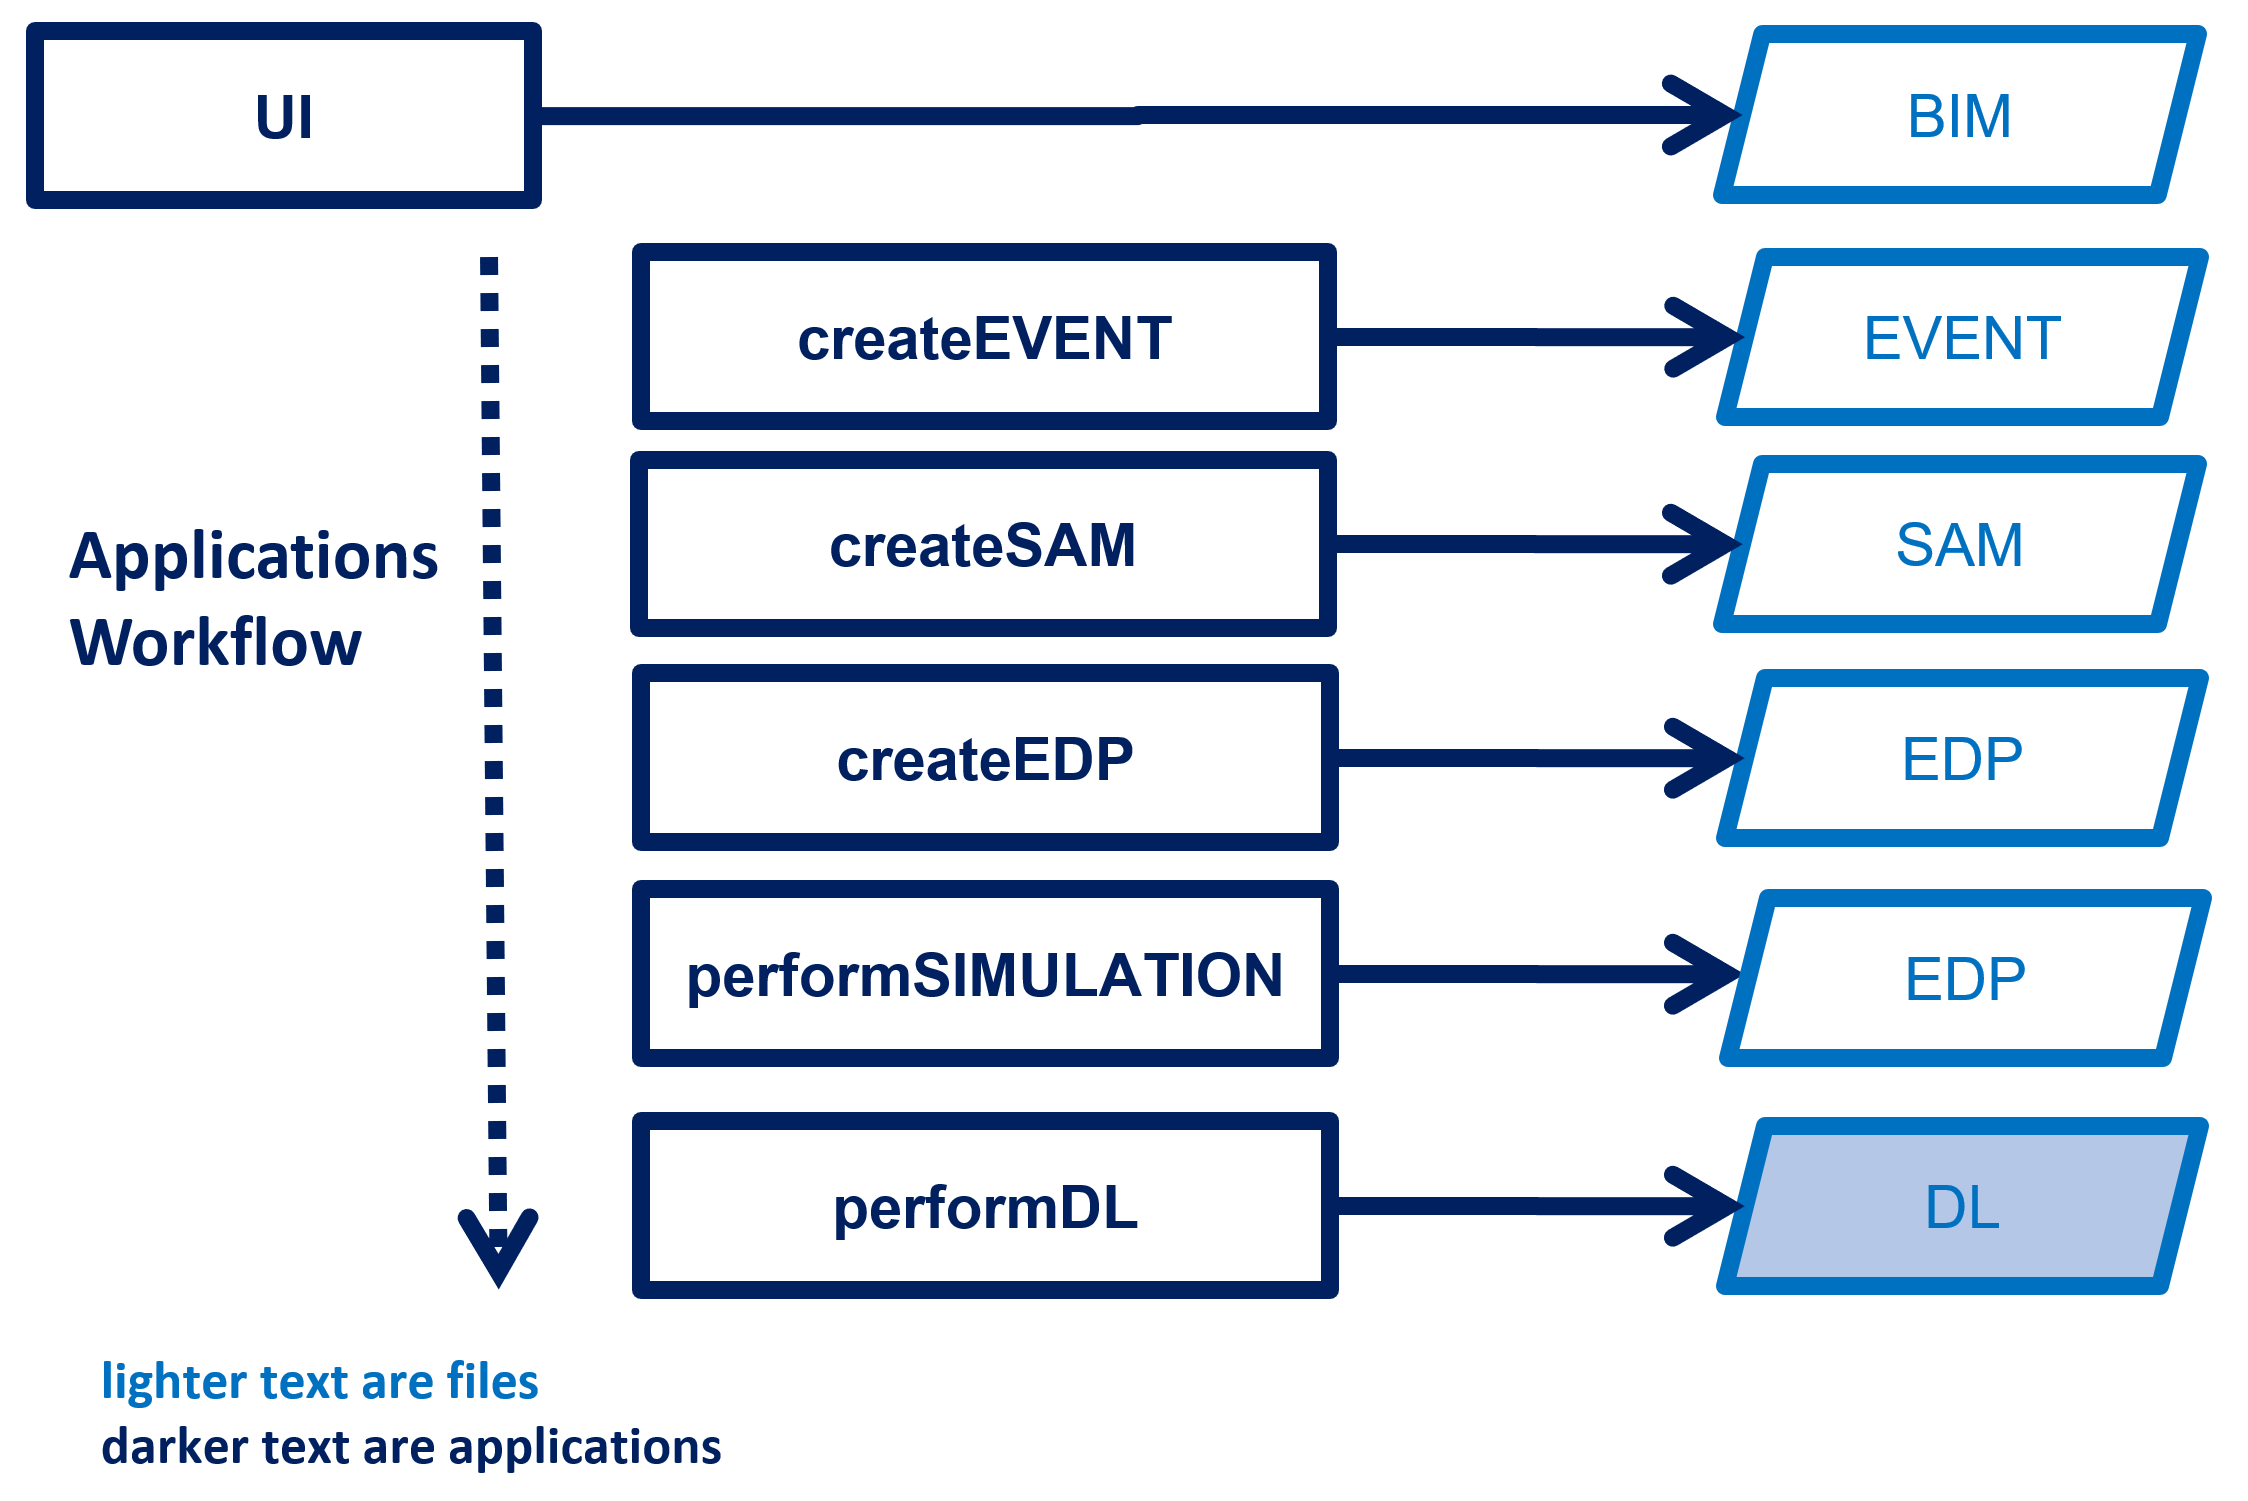
\includegraphics[width=0.6\textwidth]
        {theory_and_implementation/figures/workflow_wo_uq_PBE.png} }
      \caption{Schematic of the basic Scientific Workflow for Damage and Loss Assessment}
      \label{fig:workflow_wo_uq}
    \end{figure}
}{
    \begin{figure}[!htbp]
      \centering {
        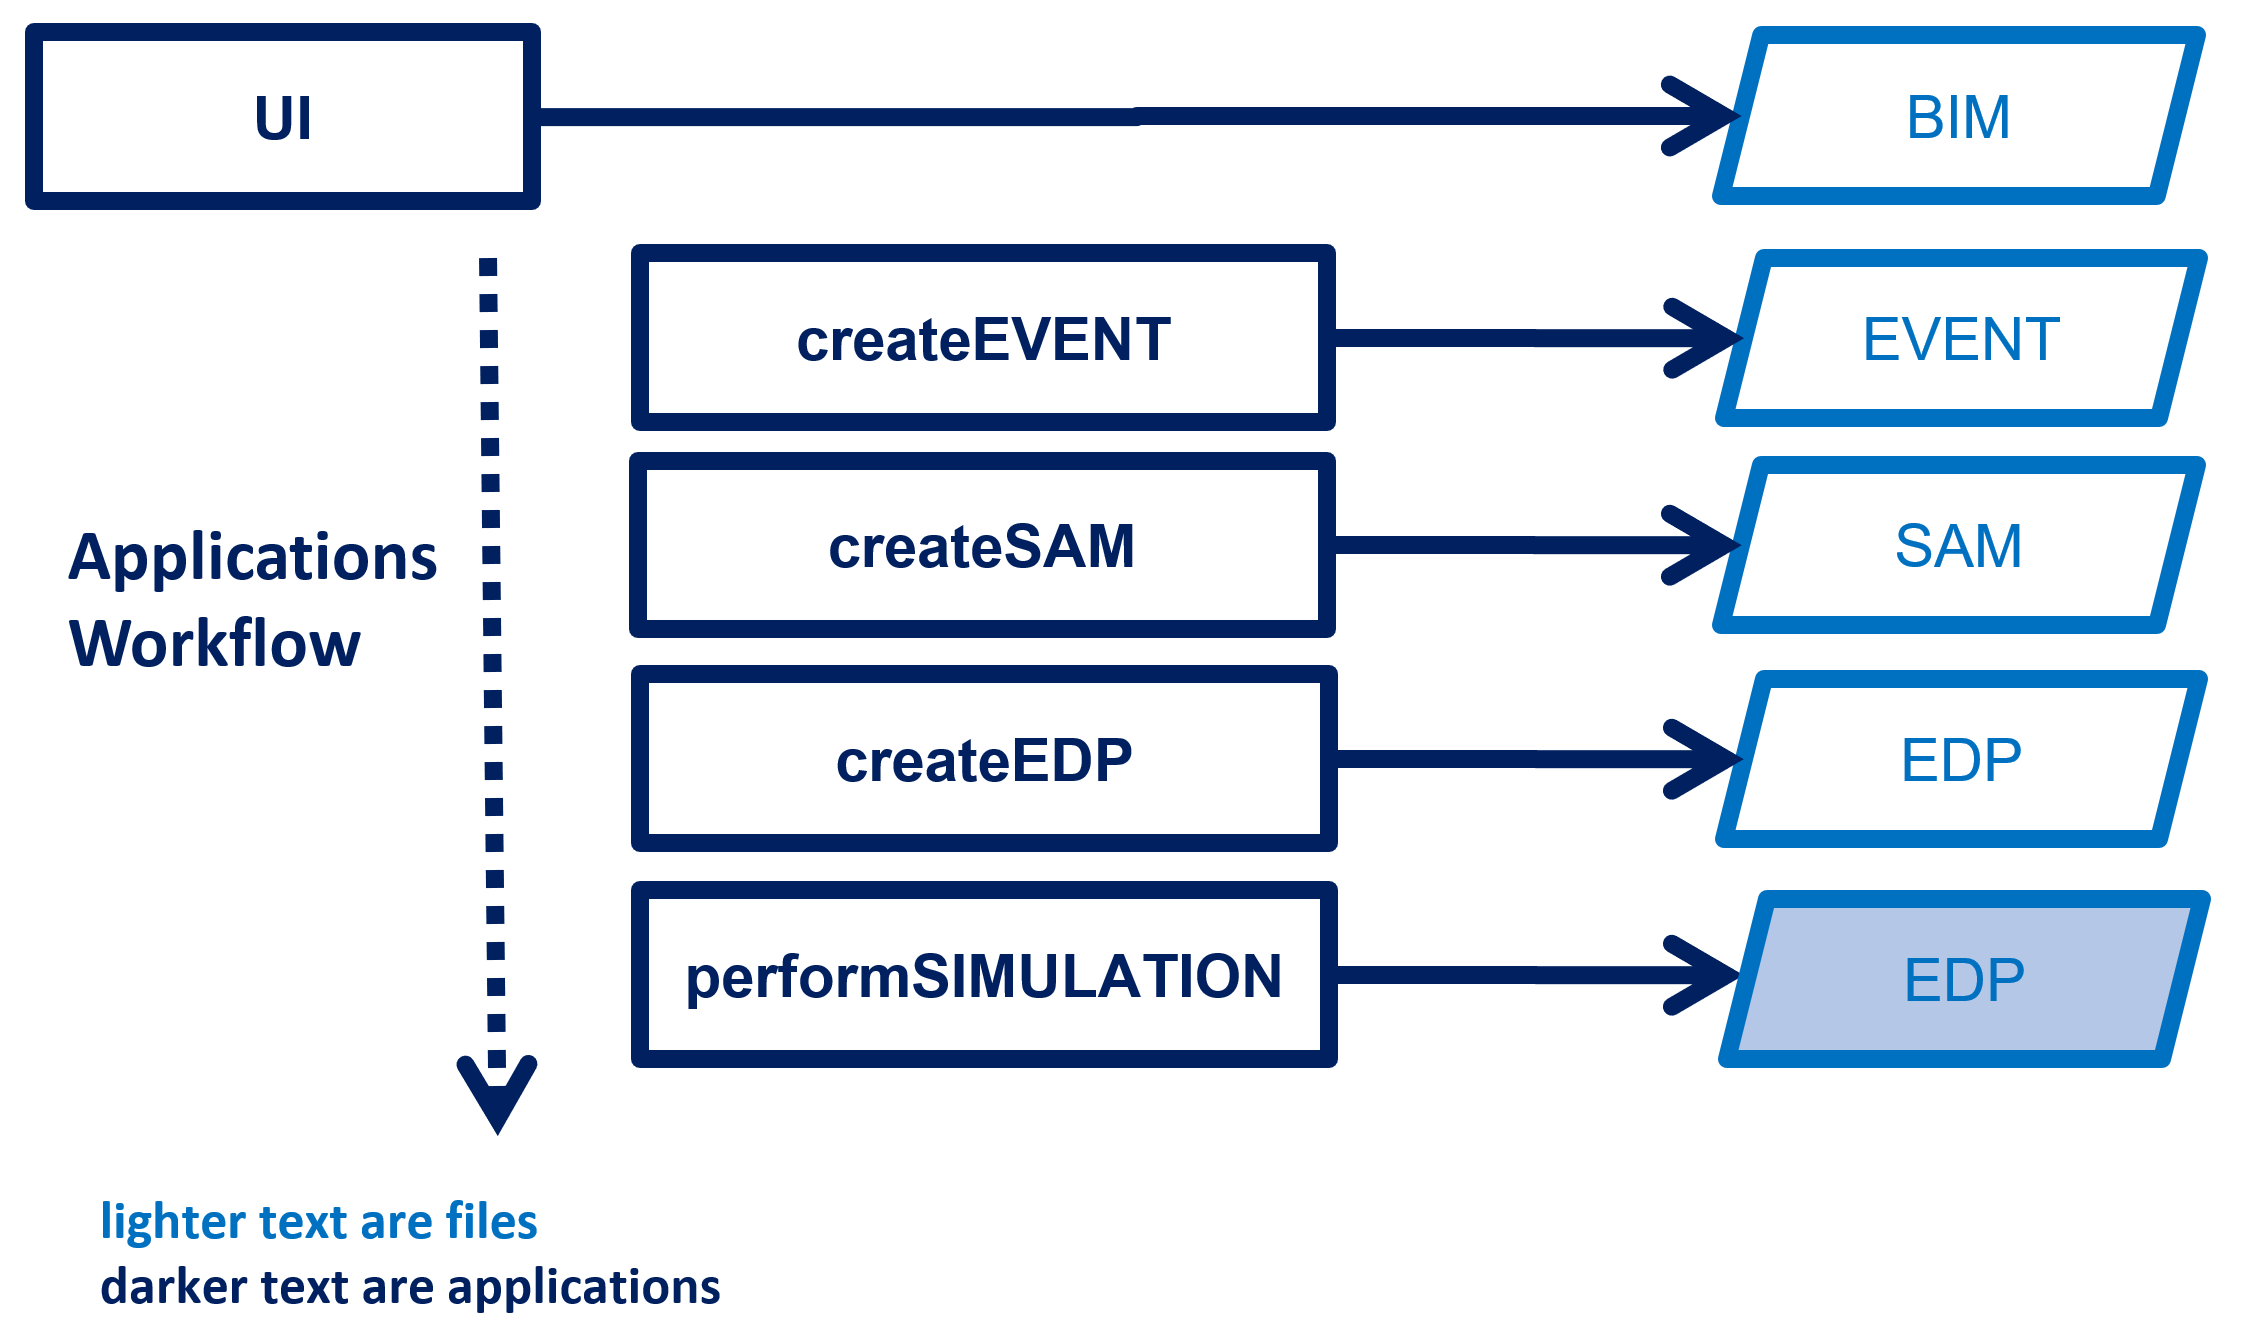
\includegraphics[width=0.6\textwidth]
        {theory_and_implementation/figures/workflow_wo_uq.png} }
      \caption{Schematic of the basic Scientific Workflow for Building Response Simulation}
      \label{fig:workflow_wo_uq}
    \end{figure}
}

The software that are invoked by the Backend Application are categorized into certain types according to their purpose:
\begin{enumerate}
    \item createEVENT: Given the structure and the user input for hazard application, define the loads for the building (i.e., the ground motion records that represent an earthquake scenario). The output file is an EVENT file.
    \item createSAM: Given the building description and event, create a response simulation model (currently, a finite element model) of the building. The output file is a SAM (Structural Analysis Model) file.
    \item createEDP: Given the building, determine what response quantities are required. The output file is the EDP (Engineering Demand Parameters) file. Currently, the user has no influence on the EDPs as the StandardEarthquakeEDP application is the built-in default application.
    \item performSIMULATION: Given the response simulation model and the event, perform a nonlinear response history simulation. The responsibility of performSIMULATION is to fill in the values in the EDP files.
\softwareSwitch{PBE}{
    \item performDL: Given the building response in the form of EDPs, perform a damage and loss assessment and provide the DVs (Decision Variables) that describe the performance of the building.
}{}
\end{enumerate}

\section{The Workflow with Uncertainty Quantification}

The need to characterize the uncertainties in the computed response complicates this workflow. All of the software above can have uncertainties in their inputs and models (e.g., building geometry or material properties in the building input file; hazard description (magnitude, distance) and corresponding ground motion records in createEVENT; finite element model parameters in createSAM; integration scheme, damping ratio or convergence tolerance in performSIMULATION, and component damage and consequence characteristics in performDL) and we want to allow users of the \texttt{\getsoftwarename{}} App to take that into consideration. \Cref{fig:uq_sampling} provides an overview of the resulting workflow with uncertainty quantification.\\

\softwareSwitch{PBE}{
    \begin{figure}[!htbp]
      \centering {
        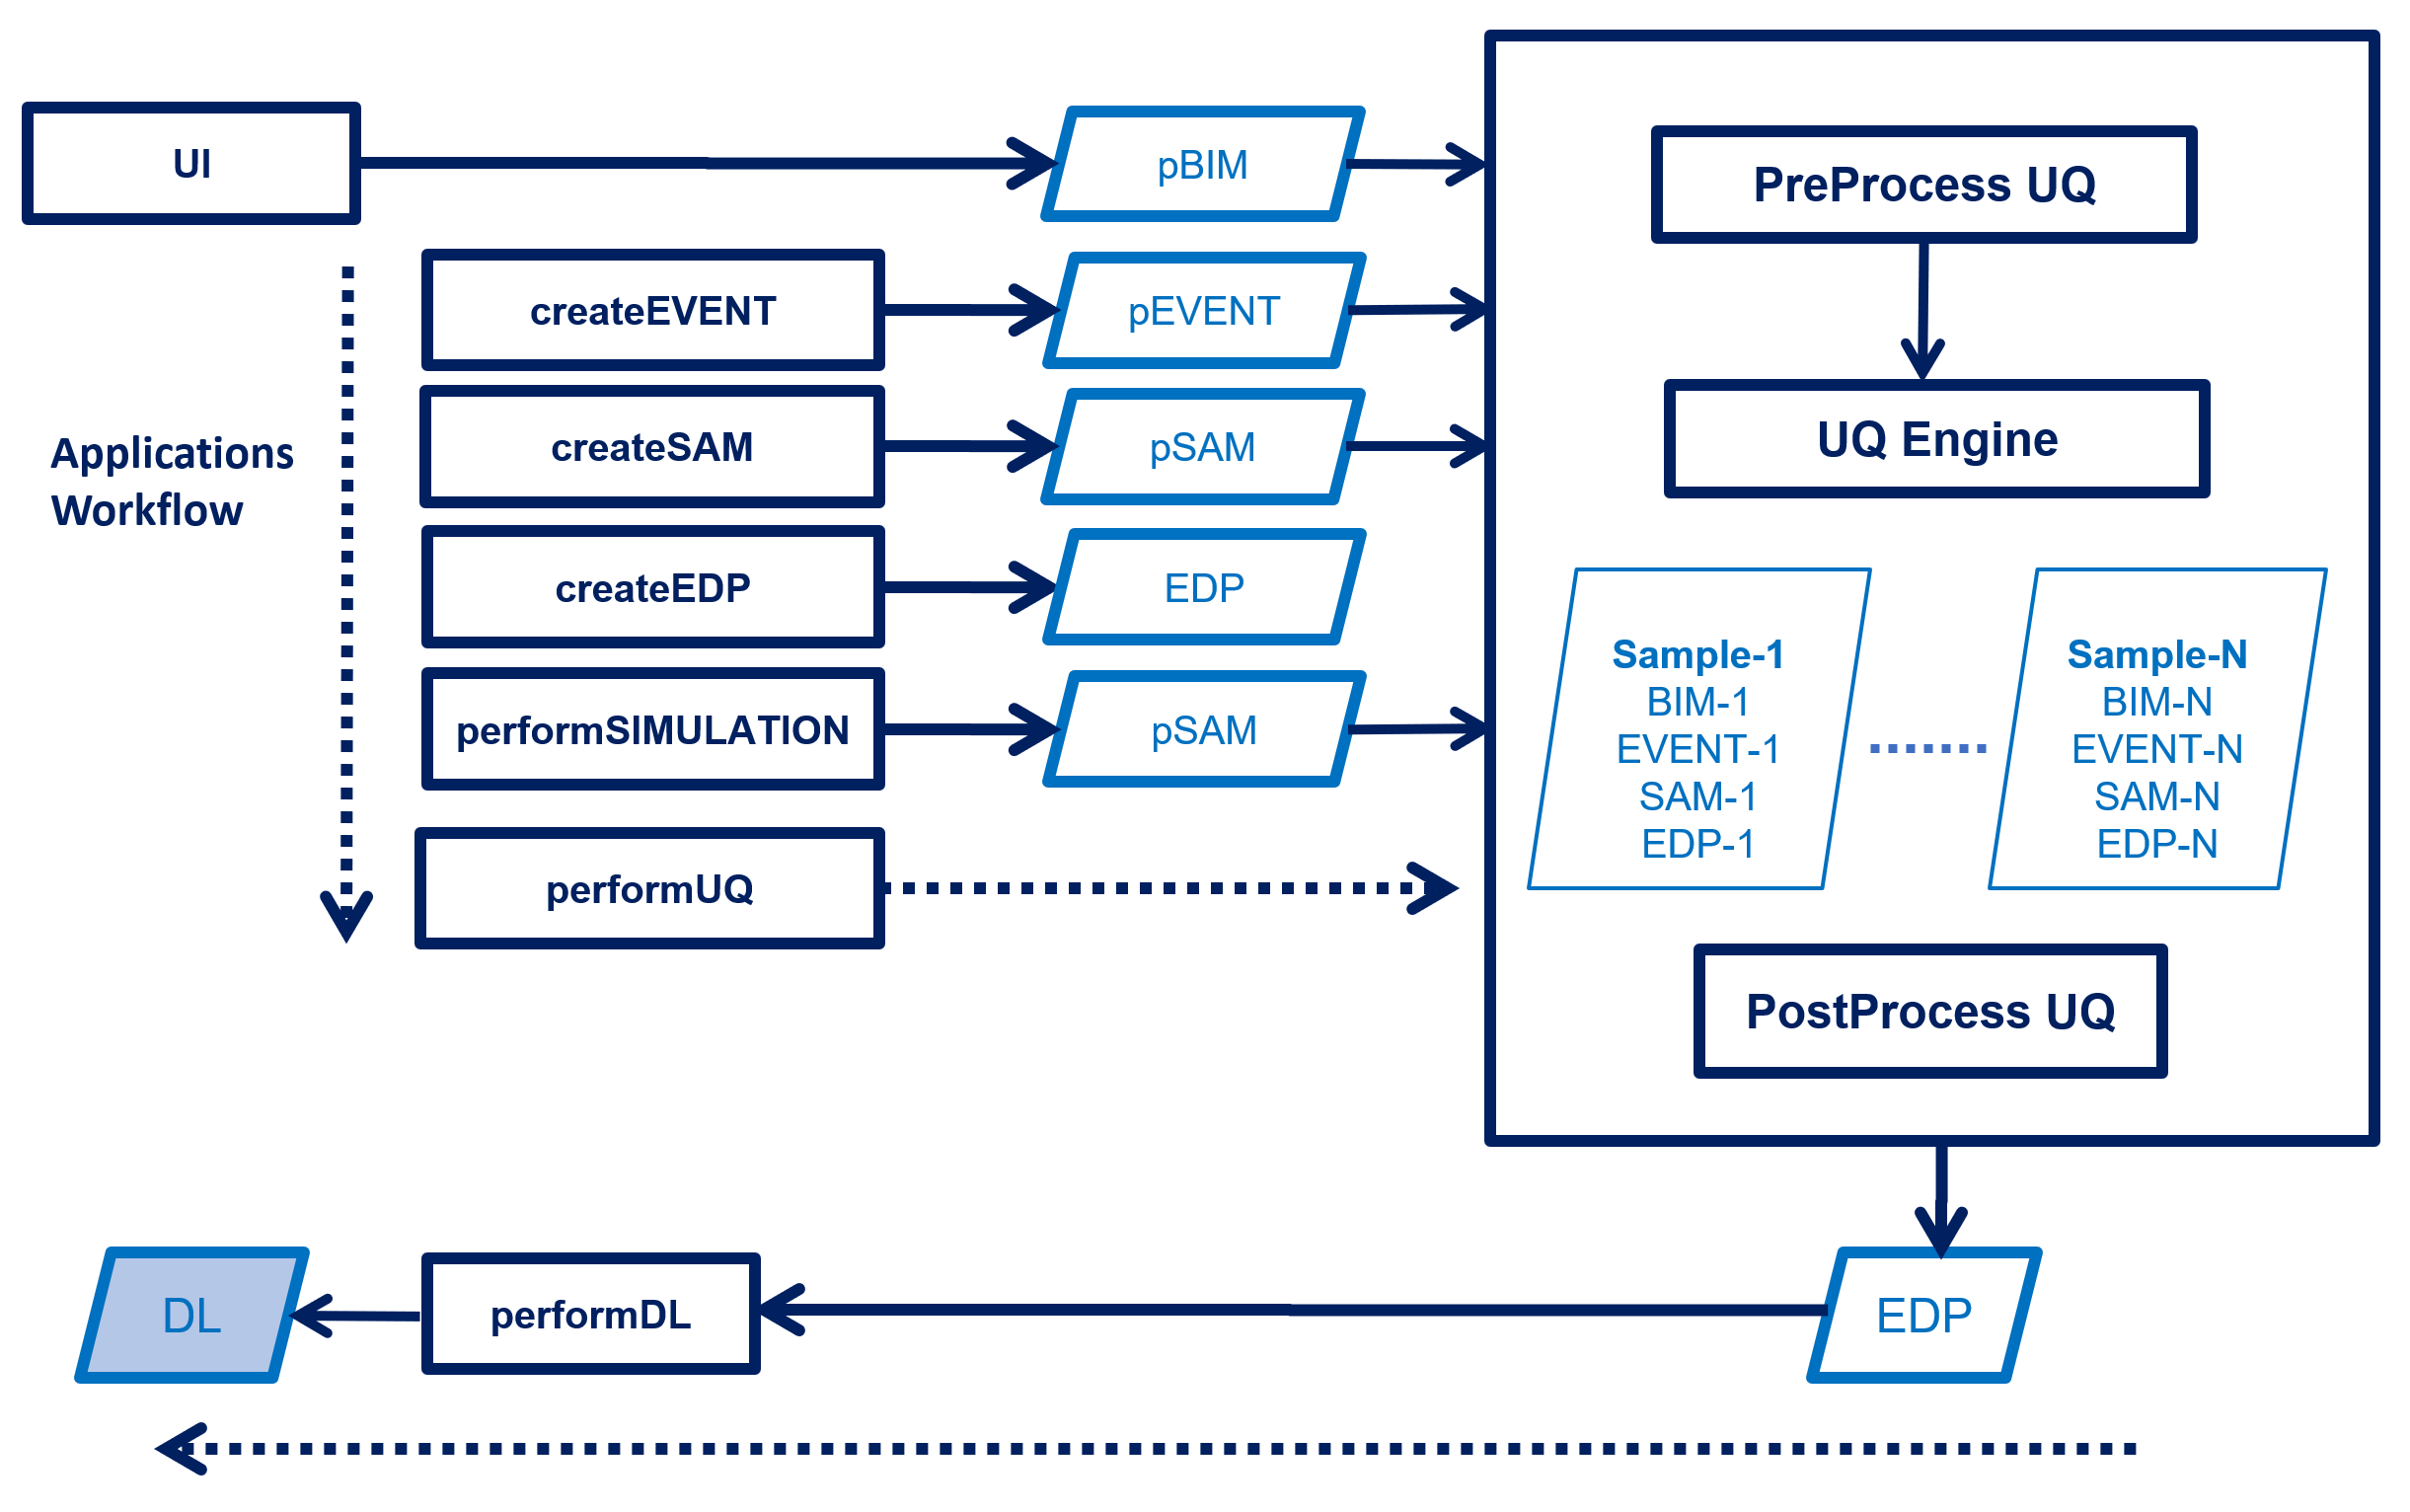
\includegraphics[width=1.0\textwidth]
        {theory_and_implementation/figures/uq_sampling_PBE.png} }
      \caption{Schematic of the Scientific Workflow Application for Damage and Loss Assessment with UQ}
      \label{fig:uq_sampling}
    \end{figure}
}{
    \begin{figure}[!htbp]
      \centering {
        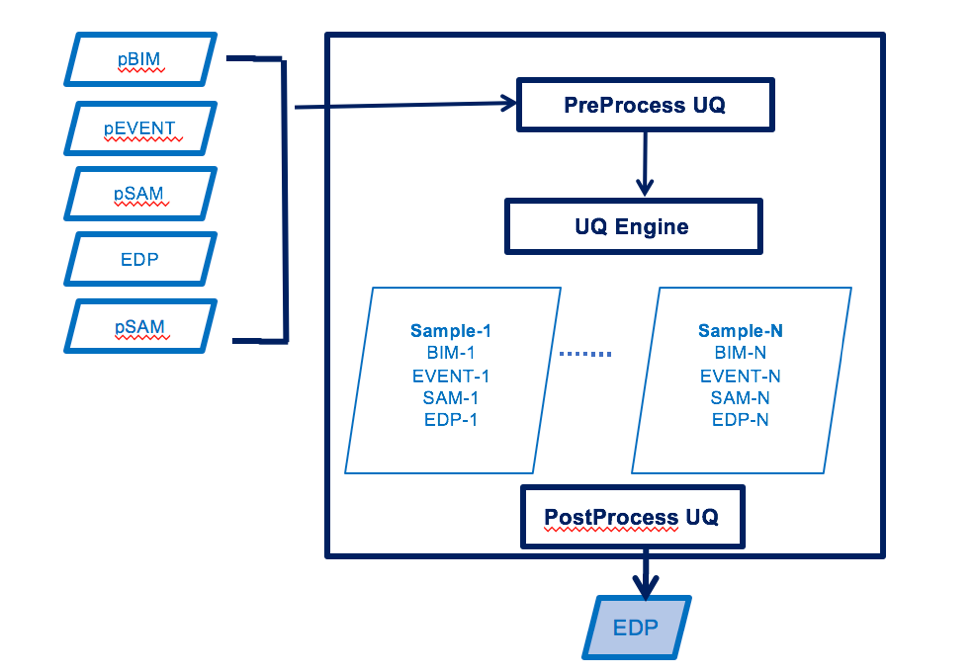
\includegraphics[width=0.8\textwidth]
        {theory_and_implementation/figures/uq_sampling.png} }
      \caption{Schematic of the Scientific Workflow Application for Building Response Simulation with UQ}
      \label{fig:uq_sampling}
    \end{figure}
}

Each application is called with two different sets of input arguments. The first time every application is called with a \texttt{–getRV} input argument. This tells them to return information about the random variables inside a \texttt{randomVariables} entry in \texttt{pFiles} (i.e., output files with a \texttt{p} prefix) generated by the application along with other needed data (e.g., the event type). The \texttt{randomVariables} is a \texttt{JSON} array of random variables, each with a field for a name, a type, a value, and other type-dependent info. A sample array is shown below with three variables:\\

\begin{lstlisting}
{
  "randomVariables": [
        {
            "distribution": "Normal",
            "mean": 6,
            "name": "fc",
            "stdDev": 0.6,
            "value": "RV.fc",
            "variableClass": "Uncertain"
        },
        {
            "distribution": "Normal",
            "mean": 60,
            "name": "fy",
            "stdDev": 6,
            "value": "RV.fy",
            "variableClass": "Uncertain"
        },
        {
            "distribution": "Normal",
            "mean": 30000,
            "name": "E",
            "stdDev": 3000,
            "value": "RV.E",
            "variableClass": "Uncertain"
        }

}
\end{lstlisting}

After preparing information about all random variables, the control of the workflow is passed to the UQ engine. It generates the prescribed number of samples of the random variables, then runs the workflow until the response simulation and collects the EDPs for each input sample. The UQ engine searches for value fields in the input files with RV.variableName values and replaces them with the realizations of the random variables.\\

The performUQ application is actually a script that calls three applications, as shown below:

\begin{enumerate}
    \item PreProcessUQ: Parses all pFiles to build the list of random variables.
    \item PerformUQ: Invokes the UQ engine, which fills in the random variable values, and runs the applications in the workflow with the updated input files.
    \item PostProcessUQ: Combines the output results, collecting the EDPs.
\end{enumerate}

The computationally expensive part of the workflow is the response simulation done by performSIMULATION within performUQ. As discussed earlier, the user has the option of running the performUQ part locally or remotely at DesignSafe. When the user selects to run the job remotely, it is only the performUQ part that runs at DesignSafe. The \texttt{pFiles} are still prepared locally. These files are placed in a directory (along with all other needed files) and transferred to DesignSafe before an Agave application is invoked to run the performUQ part of the workflow on Stampede2.

\softwareSwitch{PBE}{
The performDL part of the workflow runs separately because its stochastic loss model can be decoupled from the other parts of the workflow when analyzing single buildings. Decoupling performDL allows us to take advantage of the smaller computational burden of this part of the workflow and use a considerably larger number of samples in damage and loss calculation (i.e., 10,000 or more samples versus the typical 100 samples in response estimation).
}{}
